\documentclass[12pt]{book} 
\usepackage[utf8]{inputenc} 
\usepackage[T1]{fontenc}
\usepackage[slovene]{babel} 	
\usepackage{amsmath} 
\usepackage{amssymb} 
\usepackage{amsthm}
\usepackage{bbm}
\usepackage{lmodern}
\usepackage{graphicx}
\usepackage{tikz}
\usepackage{pgfplots}
\usepackage{enumitem}
\usepackage{biblatex}           
\usepackage{hyperref}   
\usepackage{geometry}

\usetikzlibrary{patterns}
\pgfplotsset{compat=1.17}

\geometry{
    a4paper,
    left=30mm,
    right=30mm,
    top=30mm,
    bottom=40mm
}

\makeatletter
\renewcommand{\maketitle}{
  \begin{titlepage}
    \begin{center}
      \vspace*{25mm} 
      \Huge\@title\par 
      \vspace{20mm} 
      \large\@author \\
      \vspace{140mm} 
      \large\@date\par 
    \end{center}
  \end{titlepage}
}
\makeatother

\usepackage{fancyhdr}
\pagestyle{fancy}
\fancyhf{}
\fancyhead[R]{\leftmark}
\renewcommand{\headrulewidth}{0.4pt} 
\linespread{1.3}

\usepackage{titlesec}
\titleformat{\chapter}[display]{\normalfont\Huge\bfseries}{\chaptertitlename\ \thechapter}{20pt}{\Huge}
\titleformat{\section}{\LARGE\bfseries}{\thesection}{1em}{}


\def\N{\mathbb{N}}
\def\R{\mathbb{R}}
\def\n{\noindent}
\def\s{\vspace{10pt}}


\theoremstyle{definition}
\newtheorem{definicija}{Definicija}

\theoremstyle{plain}
\newtheorem{izrek}{Izrek}

\theoremstyle{plain}
\newtheorem{trditev}{Trditev}

\theoremstyle{plain}
\newtheorem{posledica}{Posledica}

\theoremstyle{remark}
\newtheorem*{opomba}{Opomba}

\usepackage{thmtools}
\declaretheoremstyle[
    spaceabove=10pt,
    spacebelow=10pt,
    bodyfont=\normalfont,
    headfont=\bfseries,
    postheadspace=0.5em,
    qed=$\lozenge$ 
]{example}
\declaretheorem[style=example, unnumbered]{zgled}


\usepackage{filemod}
\title{\Huge Verjetnost 1}
\author{Napisal: Jon Pascal Miklavčič}
\date{\filemodprintdate{\jobname}}


\begin{document}

\frontmatter

\maketitle

\chapter*{Predgovor}
Zapiski v tej skripti so bili osnovanih na rokopisih predavanj iz študijskih let pred letom 2023 in doknčno dopolnjeni z zapiski iz predavanj iz leta 2024.

\tableofcontents

\mainmatter

\chapter{Neformalni uvod v verjetnost}

Začetki verjetnosti so v 17. stoletju, iz iger na srečo (kartanje, kockanje, \dots): 
\begin{itemize}
    \item 17. stol.: Fermant, Pascal, Bernulli;
    \item 18./19. stol.: Laplace, Poisson, Čebišev, Markov;
    \item 20. stol.: Kolmogorov.
\end{itemize}

\n Izvajamo poskus in opazujemo določen pojav, ki ga imenujemo \emph{dogodek}. Ta se lahko zgodi ali ne. 

\begin{zgled}
    Poskus je met kocke. Da pade šestica, da pade sodo število pik pa sta dogodka.
\end{zgled}

\n Poskus ponovimo $n$-krat. Opazujemo dogodek $A$. S $k_n(A)$ označimo \emph{frekvenco dogodka} $A$, t.j. število tistih ponovitev poskusa, pri katerih se je dogodek $A$ zgodil. Naj bo $f_n(A)=\frac{k_n(A)}{n}$ \emph{relativna frekvenca} dogodka $A$. Dokazati je mogoče, da zporedje $\left\{f_n(A)\right\}_n$ konvergira k nekemu številu $p \in [0, 1]$; $f_n(A) \xrightarrow{n \to \infty} p$. Dobimo:

\textbf{Statistično definicijo verjetnosti:}

$$P(A):= p $$

\n Pogosto lahko verjetnost določimo vnaprej in sicer s: 

\textbf{Klasično definicijo verjetnosti:}

$$P(A):= \frac{\# \text{ ugodnih izidov za dogodek } A}{\# \text{ vseh izidov}}$$

pri pogoju, da imajo vsi izidi \emph{enake} možnosti.

\begin{zgled}
    Met poštene kocke: 
    $$P(\text{sodo število pik}) = \frac{3}{6} = \frac{1}{2}$$
\end{zgled}

\begin{zgled}
    Kolikšna je verjetnost, da pri metu dveh poštenih kock znaša vsota pik $7$?
    
    Možne vsote so: $2, 3, 4, \dots , 12$. Opazimo, da je vseh vsot $11$ in od tega $1$ ugodna. Ali to pomeni, da $P(A)=\frac{1}{11}$. Ne! Izidi niso enkaoverjetni. 
    
    Na primer $2$ lahko dobimo samo kot $2=1+1$, $5$ pa kot $5=2+3=1+4=4+1=3+2$. 

    Torej vsi možni izidi, bodo urejeni pari $(x, y)$, kjer $x, y \in[1,6] \subset \mathbb{N}$
    $$
    \begin{array}{cccc}
        (1,1) & (1,2) & \cdots & (1,6) \\
        (2,1) & (2,2) & \ddots & (2,6)\\
        \vdots & \ddots & \ddots & \vdots \\
        (6,1) & (6,2) & \cdots & (6,6) \\
    \end{array}
    $$

    Vseh izidov je torej $36$ in od tega je $6$ ugodnih. Torej $P(A)= \frac{6}{36}=\frac{1}{6}$.
\end{zgled}

\n Če je izidov neskončno, si lahko pomagamo s \textbf{Geometrijsko definicijo verjetnosti.}

\begin{zgled}
    Osebi se dogovorita za srečanje med 10. in 11. uro. Čas prihoda je slučajen. Vsak od njiju po prihodu čaka največ 20 minut. Če v tem času drugega ni, odide. Najdlje čaka do 11. ure. Kolišna je vrejetnost srečanja?

    Čas začnemo šteti ob 10. uri. Vsi izidi so urejeni pari $(x, y) \in [0,1] \times[0,1]$. Ugodni izidi so $|x-y| \leq \frac{1}{3}$. Torej: 
    $$
    \begin{aligned}
        \text{1) } x \geq y &: x-\frac{1}{3} \leq y \\
        \text{2) } x \leq y &: y-x \leq \frac{1}{3} \iff y \leq x+\frac{1}{3}
    \end{aligned}
    $$

    Torej je $$P(\text{srečanja})=\frac{1-\left(\frac{2}{3}\right)^2}{1}=\frac{5}{9}$$
\end{zgled}

\n Teorija mere se ukvarja z splošnim zapisom geometrijske definicije. 

\begin{zgled}
    Vzamemo $m, n \in \mathbb{N}$, $m>n$. $n$ krogljic slučajno razporedimo v $m$ posod. Kolikšna je verjetnost dogodka, da so vse krogljice v prvih $n$ posodah, v vsaki ena?

    To je pomankljivo zastavljena naloga. Ne vemo namreč, ali med seboj krogljice razlikujemo, ali ne. Za dodatno predpostavko se ponujajo 3 možnosti: 

    1) \textbf{krogljice razlikujemo:}
    
    \n Število vseh izidov v tem primeru je ravno število \emph{variacij} $m$ elementov na $n$ mestih \emph{s ponavljanjem}. Za vsako od $n$-tih kroglic imamo $m$ možnosti, torej je vseh možnosti $m \cdot m \cdots m=m^n$.
    
    \n Število ugodnih izidov pa je ravno število \emph{permutacij} $n$ krogljic v prvih $n$ posodah. Torej je ugodnih možnosti $n(n-1) \ldots 2 \cdot 1=n!$.
    
    Torej je $$P(A)=\frac{n !}{m^n}$$

    2) \textbf{krogljic ne razlikujemo:} 
    
    \n V vsaki posodi je lahko več krogljic. Število vseh izidov je ravno število \emph{kombinacij s ponavljanjem}. Število kombinacij $m$ elementov s ponavljanjem na $n$ mestih je: 
    $$
    \binom{n+m-1}{n} = \binom{n+m-1}{m-1}
    $$

    \n Postavimo $n$ krogljic in med njih razporedimo $m-1$ črtic, ki predstavljajo stene posod:
    $$
    |\underbrace{\circ|\circ|\circ\circ |\circ\circ  \cdots |\circ |}_{n \text{ krogljic, } m-1 \text{ črtic}}|
    $$

    \n Na $n+m-1$ mestih moramo določiti $n$ krogljic. Ugoden izid je samo eden: 
    $$
    |\circ|\circ|\circ|\circ \cdots \circ|||| \cdots |
    $$

    Torej je $$P(A)=\frac{1}{\binom{n+m-1}{n}}$$

    3) \textbf{krogljic ne razlikujemo, v vsaki posodi je kvečjemu ena krogljica:} 
    
    Število vseh izidov je ravno število \emph{kombinacij brez ponavljanja} $\binom{m}{n}$. Ugoden izid je eden. 

    Torej je $$P(A)=\frac{1}{\binom{m}{n}}$$
\end{zgled}

\begin{opomba}
V fiziki so krogljice delici (atomi, molekule, ...), posode pa fazna stanja, v katerih so lahko delci. Glede na zgornje primere ločimo:

\begin{enumerate}
    \item Maxwell-Boltzmannovo statistika, ki velja za molekule plina.
    \item Bose-Einsteinovo statistika, ki velja za delce imenovane bozoni.
    \item Fermi-Diracovo statistika, ki velja za fermione. 
\end{enumerate}

\n Diracovo izključitveno načelo.

\end{opomba}

\newpage

\chapter{Aksiomatična definicija verjetnosti}

Imamo prostor vseh izidov oz. \emph{vzorčni prostor} $\Omega$ (možna oznaka je tudi $\mathcal{G}$). Dogodki so nekatere (ne nujno vse) podmnozice $\Omega$.

\begin{zgled}
    Met kocke. Vzorčni prostor je $\Omega=\{1,2,3,4,5,6\}$, dogodki pa so poljubne podmnožice $\Omega$, to je $\mathcal{P}(\Omega) = 2^{\Omega}$. Na primer $A = \{2,4,6\}$ je dogodek, da pade sodo število pik. 
\end{zgled}

\n Računanje z dogodki:

\begin{enumerate}
    \item \emph{Vsota dogodkov} oz. \emph{unija dogodkov} (zgodi se vsaj enden od dogodkov): $$A + B = A \cup B$$
    \item \emph{Produkt dogodkov} oz. \emph{presek dogodkov} (zgodita se oba dogodka hkrati): $$A \cdot B = A \cap B$$
    \item \emph{Nasprotni dogodek} oz. \emph{komplement dogodka} (dogodek se ne zgodi): $$\bar A = A^c$$
\end{enumerate}

\n Pravila za računanje z dogodki: 

\begin{enumerate}
    \item \textbf{idempotentnost}: $A \cup A=A=A \cap A$
    \item \textbf{komutativnost}: $A \cup B=B \cup A, \quad A \cap B=B \cap A$
    \item \textbf{asociativnost}: $$\begin{aligned} & (A \cup B) \cup C=A \cup(B \cup C) \\ & (A \cap B) \cap C=A \cap(B \cap C)\end{aligned}$$
    \item \textbf{distributivnost}: $$\begin{aligned} & (A \cup B) \cap C=(A \cap C) \cup(B \cap C) \\ & (A \cap B) \cup C=(A \cup C) \cap(B \cup C)\end{aligned}$$
    \item \textbf{de Morganova zakona}: $$\begin{aligned} & (A \cap B)^c=A^c \cup B^c \\ & (A \cup B)^c=A^c \cap B^c\end{aligned}$$ \\ Še več: $$ \left(\bigcap_i A_i\right)^c=\bigcup_i A_i^c, \quad \left(\bigcup_i A_i\right)^c=\bigcap_i A_i^c$$
\end{enumerate}

\n V splošnem ni vsaka podnožica množice $\Omega$ dogodek. Neprazna družina podmnožic (dogodkov) $\mathcal{F}$ v $\Omega$ je \emph{$\sigma$-algerba}, če zanjo velja: 

\begin{enumerate}
    \item $\Omega \in \mathcal{F}$
    \item $A \in \mathcal{F} \implies A^c \in \mathcal{F}$
    \item $A_1, A_2, \ldots \in \mathcal{F} \implies \bigcup_{i=1}^{\infty} A_i \in \mathcal{F}$
\end{enumerate}

\n Elementi v $\mathcal{F}$ so dogodki. Če v točki 3. zahtevamo manj: 

\begin{enumerate}[start=3,label={\arabic*.*}]
    \item $A, B \in \mathcal{F} \implies A \cup B \in \mathcal{F}$
\end{enumerate}

potem pravimo, da je $\mathcal{F}$ \emph{algebra}. \s

V algebri imamo potem tudi zaprtost za končne unije: $A_1, A_2, \ldots, A_n \in \mathcal{F} \implies A_1 \cup A_2 \cup \cdots \cup A_n \in \mathcal{F}$. Ker po de-Morganu velja $\bigcap_i A_i=\left(\bigcup_i A_i^c\right)^c$, je algebra zaprta za končne preseke, $\sigma$-algebra pa celo za števne preseke. Ker velja $A \setminus B=A \cap B^c$, je algebra zaprta za razlike. 

Vsaka algebra vsebuje $\{\emptyset, \Omega\}$. Ker je $\mathcal{F}$ neprazna, obstaja $A \in \mathcal{F}$ in zato tudi $\Omega=A \cup A^c \in \mathcal{F}$ in $\emptyset=\Omega^c \in \mathcal{F}$. Tako dobimo, da je $\{\emptyset, \Omega\}$ najmanšja možna ($\sigma$-)algebra, $\mathcal{P}(\Omega)$ pa največja možna ($\sigma$-)algebra.

\begin{zgled}
    Za $A \neq \emptyset \neq \Omega$ je najmanjša ($\sigma$-)algebra, ki vsebuje $A$ enaka $\left\{\emptyset, A, A^c, \Omega\right\}$. 

    \n Za $\Omega=\{1,2,3\}$ in $A=\{1,2\}$, je potem taka $\sigma$-algebra $\{\emptyset,\{3\},\{1,2\},\{1,2,3\}\}$.
\end{zgled}

Dogodka $A$ in $B$ sta \emph{disjunkta} oz. \emph{nezdružljiva} če je $A \cap B=\emptyset$. 

Zaporedje $\{A_i\}_i$ (končno ali števno mnogo) je \emph{popoln sistem dogodkov}, če velja: $$\bigcup_i A_i=\Omega \quad \text{in} \quad A_i \cap A_j = \emptyset \quad \text{za} \quad i \neq j.$$ 

\n Naj bo $\mathcal{F}$ $\sigma$-algebra na $\Omega$. \textbf{Verjetnost} na $(\Omega, \mathcal{F})$ je preslikava $P:\mathcal{F} \to \mathbb{R}$ z lastnostmi:

\begin{enumerate}
    \item Za vsak $A \in \mathcal{F}$: $P(A) \geq 0 $
    \item $P(\Omega) = 1$
    \item Za poljubne paroma nezdružljive dogodke $\{A_i\}_{i=1}^{\infty}$ velja števna aditivnost: $$P\left(\bigcup_{j=1}^{\infty} A_i\right)=\sum_{i=1}^{\infty} P\left(A_i\right)$$
\end{enumerate}

\n Lastnosti verjetnosti $P$: 

\begin{enumerate}[label=(\alph*)]
    \item $P(\emptyset) = 0$. 
    \begin{proof}
        V lastnosti 3. vzamamo $A_i = \emptyset$ za vsak $i$: 
        $$
        P\left(\bigcup_i \emptyset\right)=P(\emptyset)+P(\emptyset)+P(\emptyset)+\cdots = 0+0+0+ \cdots = 0
        $$
    \end{proof}
    \item $P$ je \emph{končno aditivna}, t.j. za končno mnogo paroma nezdružljivih dogodkov $\{A_i\}_{i=1}^{n}$ velja: 
    $$
    P\left(A_1 \cup \cdots \cup A_n\right)=P\left(A_1\right)+P\left(A_2\right)+\cdots+P\left(A_n\right)
    $$
    \begin{proof}
        V lastnosti 3. vzamemo $A_{n+1}=A_{n+2}=\cdots=\emptyset$ in upoštevamo lastnost (a). 
    \end{proof}
    \item $P$ je \emph{monotona}, t.j. velja: 
    $$
    A \subseteq B \implies P(A) \leq P(B)
    $$ 
    Še več: iz $A \subseteq B$  sledi $P(B \setminus A)=P(B)-P(A)$.
    \begin{proof}
        Ker je $B=A \cup(B \setminus A)$ in $A \cap(B \setminus A)=\emptyset$ je $P(B)=P(A)+P(B \setminus A)$ zaradi lastnosti (b).
    \end{proof}
    \item $P(A^c) = 1-P(A)$
    \begin{proof}
        V (c) vzamemo $B = \Omega$.
    \end{proof}
    \item $P$ je \emph{zvezna}, t.j.:
    
    \begin{enumerate}[label=(\roman*)]
        \item $$ A_1 \subseteq A_2 \subseteq A_3 \subseteq \cdots \implies P\left(\bigcup_{i=1}^{\infty} A_i\right)=\lim _{n \to \infty} P\left(A_n\right)$$
        \item $$ B_1 \supseteq B_2 \supseteq B_3 \supseteq \cdots \implies P\left(\bigcap_{i=1}^{\infty} B_i\right)=\lim _{n \to \infty} P\left(B_n\right)$$
    \end{enumerate}

    \begin{proof}
        \begin{enumerate}[label=(\roman*)]
            \item Definiramo $C_1 = A$ in $C_i = A_i \setminus A_{i-1}$ za $i = 2, 3, \ldots$. Potem je $A_n=C_1 \cup \ldots \cup C_n$, kjer velja $C_i \cap C_j=\emptyset$ za $i \neq j$ in $\bigcup_{i=1}^{\infty} A_i=\bigcup_{i=1}^{\infty} C_i$. Torej je: 
            $$ \begin{aligned} P\left(\bigcup_{i=1}^{\infty} A_i \right) &= P\left(\bigcup_{i=1}^{\infty} C_i\right) \\ &= \sum_{i=1}^{\infty} P(C_i) \\ &= \lim _{n \to \infty} \sum_{i=1}^{n} P(C_i) \\ &= \lim _{n \to \infty} P\left(\bigcup_{i=1}^n C_i\right) \\ &= \lim_{n \to \infty} P(A_n) \end{aligned}$$ 
            \item Ker $B_1 \supseteq B_2 \supseteq B_3 \supseteq \cdots$, je potem $B_1^c \subseteq B_2^c \subseteq B_3^c \subseteq \cdots$. Po (i) potem velja 
            $$P\left(\bigcup_{i=1} B_i^c\right)=\lim _{i \to \infty} P\left(B_i^c\right)$$ 
            Toda $$ \bigcup_{i=1}^{\infty} B_i^c=\left(\bigcap_{i=1}^{\infty} B_i\right)^c \implies 1-P\left(\bigcap_{i=1}^{\infty} B_i\right)=\lim_{i \to \infty}\left(1-P(B_i\right)) $$ Od koder sledi željena enakost. 
        \end{enumerate}
    \end{proof}
\end{enumerate}

\textbf{Verjetnostni prostor} je trojica $(\Omega, \mathcal{F}, P)$

\begin{zgled}[Končni ali števni verjetnostni prostor]
    $\Omega=\left\{\omega_2, \omega_2, \omega_3, \ldots\right\}$ končno ali števno mnogo izidov. $\left\{\omega_1\right\},\left\{\omega_2\right\},\left\{\omega_3\right\}, \ldots$ je popoln sistem dogodkov, neka podmnožica v $\Omega$ je končna ali števna unija teh dogodkov. Torej $\mathcal{F}=\mathcal{P}(\Omega)$. Vzamemo:
    $$
    A=\bigcup_{i: \omega_i \in A}\left\{\omega_0\right\} 
    $$
    Če označimo $P(\{\omega_i\}) = p_i \geq 0$ je $\sum_i p_i=1$ in $P(A)=\sum_{i: \omega_i \in A} p_i$, $A \subseteq \Omega$.

    Če ima $\Omega$ $n$ elementov in $p_i = \frac{1}{n}$ za $i=1, 2, \ldots, n$. Potem je $P(A)=\frac{|A|}{n}=\frac{\operatorname{moč}(A)}{n}$. To je klasična definicija verjetnosti. 
\end{zgled}

\begin{zgled}[Neskončni neštevni verjetnostni prostor]
    Primer srečanja dveh oseb, kjer $\Omega=[0,1] \times[0,1]$. Za $\sigma$-algebro $\mathcal{F}$ ne moremo vzeti vseh podmnožic, radi pa bi jih vzeli čim več.

    $\mathcal{F}$ naj bo najmanjša $\sigma$-algebra, ki vsebje vse odprte pravokotnike $(a, b)\times(c, d)$ (izkaže se, da je isto, če vzamemo zaprte pravokotnike). $\mathcal{F}$ imenujemo \emph{Borelova $\sigma$-algebra}.

    Verjetnost definiramo na pravokotnikih kot: 
    $$
    P((a, b) \times(c, d))=(b-a)(d-c)
    $$
    Ni lahko videti, da lahko $P$ razširimo do verjetnosti na $\mathcal{F}$. $P$ pa ne moremo razširiti na $\mathcal{P}(\Omega)$. Problem je števna aditivnost. 

    To je geometrijska definicija verjetnosti.
\end{zgled}

\chapter{Pogojna verjetnost}

Naj bo $(\Omega, \mathcal{F}, P)$ verjetnostni prostor. Fiksirajmo dogodek $B$ s $P(B) > 0$. \emph{Pogojna verjetnost} dogodka $A$ glede na dogodek $B$ je: 
$$
P(A \mid B)=\frac{P(A \cap B)}{P(B)}
$$

\begin{zgled}
    V posodi sta dve beli in ena črna krogljica. Dvakrat zaporedoma izvlečemo krogljico. Kolikšna je verjetnost, da smo drugič izbrali belo krogljico, če smo prvič izbrali belo?

    \begin{enumerate}[label=(\alph*)]
        \item Krogljice vrečamo.
        
        Vseh izidov je 9: 
        $$
        \begin{array}{ccc}
            B_1 B_1 & B_1 B_2 & B_1 Č \\
            B_2 B_1 & B_2 B_2 & B_2 Č \\
            Č B_1 & Č B_2 & Č Č
        \end{array}
        $$
        \begin{flalign*}
            &\quad P(\text{prvič belo}) = \frac{6}{9} = \frac{2}{3} & \\
            &\quad P(\text{prvič in drugič belo}) = \frac{4}{9} & \\
            &\quad P(\text{drugič belo | prvič belo}) = \frac{4 / 9}{6 / 9}=\frac{4}{6}=\frac{2}{3} & \\
            &\quad P(\text{drugič belo}) = \frac{6}{5}=\frac{2}{3} & 
        \end{flalign*}

        \item Krogljic ne vračamo. 
        
        Vseh izidov je 6: 
        $$
        \begin{array}{cccccc}
            B_1 B_2 & B_1 Č & B_2 B_1 & B_2 Č & Č B_1 & Č B_2 
        \end{array}
        $$
        \begin{flalign*}
            &\quad P(\text{prvič belo}) = \frac{4}{6} = \frac{2}{3} & \\
            &\quad P(\text{prvič in drugič belo}) = \frac{2}{6} = \frac{1}{3} & \\
            &\quad P(\text{drugič belo | prvič belo}) = \frac{2 / 6}{4 / 6}=\frac{1}{2}=\frac{2}{4} & \\
            &\quad P(\text{drugič belo}) = \frac{4}{6}=\frac{2}{3} & 
        \end{flalign*}
    \end{enumerate}
\end{zgled}

\n Iz definicije pogojne verjetnosti dobimo:
$$
P(A \cap B)=P(A \mid B) \cdot P(B)  
$$

\n Za 3 dogodke $A, B, C$, kjer velja $P(B \cap C)>0$ dobimo:
$$
P(A \cap B \cap C)=P(A \mid B \cap C) \cdot P(B \cap C)=P(A \mid B \cap C) \cdot P(B \mid C) \cdot P(C)
$$

\n Če to posplošimo na $n$ dogodkov dobimo: 
$$
P\left(A_1 \cap A_2 \cap \cdots \cap A_n\right) =P\left(A_1\right) \cdot P\left(A_2 \mid A_1\right) \cdots P\left(A_n \mid A_1 \cap \cdots \cap A_{n-1}\right) 
$$

Če desno stran razpišemo, res dobimo: 
$$
\begin{aligned}
    P\left(A_1 \cap A_2 \cap \cdots \cap A_n\right) &=P\left(A_1\right) \cdot P\left(A_2 \mid A_1\right) \cdots P\left(A_n \mid A_1 \cap \cdots \cap A_{n-1}\right) \\
    &=P\left(A_1\right) \cdot \frac{P\left(A_1 \cap A_2\right)}{P\left(A_1\right)} \cdots \frac{P\left(A_1 \cap \cdots \cap A_n\right)}{P\left(A_1 \cap \cdots \cap A_{n-1}\right)} \\
    &=P\left(A_1 \cap A_2 \cap \cdots \cap A_n\right)
\end{aligned}
$$

\begin{zgled}
    V posodi imamo 6 modrih, 5 rdečih in 4 zelene krogljice. Brez vračanja izberemo 3 krogljice. Kolikšna je verjetnost, da so vse rdeče?

    Označimo s $A_k$ dogodek, da je $k$-ta krogljica rdeče za $k=1, 2, 3$. Nalogo laho rešimo na dva načina:

    \begin{enumerate}
        \item 
        $$
        \begin{aligned}
            P\left(A_1 \cap A_2 \cap A_3\right) &=P\left(A_1\right) \cdot P\left(A_2 \mid A_1\right) \cdot P\left(A_3 \mid A_1 \cap A_2\right) \\
            &=\frac{5}{15} \cdot \frac{4}{14} \cdot \frac{3}{13}=\frac{2}{7 \cdot 13}=\frac{2}{91}
        \end{aligned}
        $$
        \item $$ P(\text{vse rdeče}) = \frac{\binom{5}{3}}{\binom{15}{3}}=\frac{\frac{5 \cdot 4 \cdot 3}{3 !}}{\frac{15 \cdot 14 \cdot 13}{3 !}}=\frac{2}{91} $$
    \end{enumerate}
\end{zgled}

\n Imejmo poskus, ki ga opravimo v 2 korakih (fazah). 

\begin{enumerate}
    \item V prvem koraku se zgodi natanko enden izmed paroma nezdružljivih dogodkov $H_1, H_2, H_3, \ldots $ (končno ali števno mnogo). 
    \item V drugem koraku pa nas zanima dogodek $A$. Izrazimo $P(A)$ z verjetnostmi: $$P\left(H_i\right) \quad \text{in} \quad P\left(A \mid H_i\right) \quad \text{za} \; i= 1, 2, 3, \ldots $$
\end{enumerate}

Ker je $\{ H_i \}_i$ popoln sistem dogodkov, je:
$$
A=A \cap \Omega=A \cap\left(\bigcup_i H_i\right)=\bigcup_i A \cap H_i
$$

in zato
$$
P(A)=\sum_i P\left(A \cap H_i\right)=\sum_i P\left(H_i\right) \cdot P(A \mid H_i)
$$
To je \textbf{formula za popolno verjetnost}.

\begin{zgled}
    Pri srečolovu je $n$ srečk, od tega je $m$ dobitnih ($m<n$). Ali imamo večje možnosti za dobitek, če izbiramo prvi ali drugi?

    Če izbiramo prvi je:
    $$
    P(\text{dobitka}) = \frac{m}{n}
    $$

    Če izbiramo drugi je:
    $$
    \begin{aligned}
        P(\text{dobitka}) &= P(\text{prvi dobi}) \cdot P(\text{dobitka | prvi dobi}) \\
        & \qquad + P(\text{prvi ne dobi}) \cdot P(\text{dobitka | prvi ne dobi}) \\
        &= \frac{m}{n} \cdot \frac{m-1}{n-1}+\frac{n-m}{n} \cdot \frac{m}{n-1} =\frac{m}{n}
    \end{aligned}
    $$
\end{zgled}

\n Pogosto nas v dvofaznem poskusu  zanima: 
$$
P\left(H_k \mid A\right)=\frac{P\left(H_k \cap A\right)}{P(A)}=\frac{P\left(H_k\right) \cdot P\left(A \mid H_k\right)}{\sum_i P\left(H_i\right) \cdot P\left(A \mid H_i\right)}
$$
To je \textbf{Bayesova formula}.

\begin{zgled}
    Test s poligrafom (detektorjem laži). Resnicoljub opravi test s poligrafom z verjetnostjo $0.95$. Z enako verjetnostjo poligraf prepozna lažnivca. Izmed 1000 oseb, med kateremi je natanko en lažnivec, slučajno izberemo eno osebo za katero poligraf pravi, da je lažnivec. Kolikšna je pogojna verjetnost, da je oseba zares lažnivec?

    Označimo s $L$ dogodek, da je izbrana oseba lažnivec, $L_p$ pa dogodek, da poligraf za osebo pravi, da je lažnivec. Potem:
    $$
    P\left(L_p \mid L\right)=0.95, \quad  P\left(L_p \mid L^c\right)=0.05 \quad \text{in} \quad P(L)=0.001
    $$

    Zanima nas $P\left(L \mid L_p\right)$. Po Bayesovi formuli je:
    $$
    \begin{aligned}
        P\left(L \mid L_p\right)&=\frac{P(L) \cdot P\left(L_p \mid L\right)}{P(L) \cdot P\left(L_p \mid L\right)+P\left(L^c\right) \cdot P\left(L_p \mid L^c\right)} \\
        &=\frac{0.55 \cdot 0.001}{0.55 \cdot 0.001+0.05 \cdot 0.999} \\
        &=\frac{95}{5090} = \frac{1}{50} = 0.02 
    \end{aligned}
    $$
\end{zgled}

\n Dogodka $A$ in $B$ sta \emph{neodvisna}, če velja: 
$$
P(A \cap B)=P(A) \cdot P(B)
$$
Če je $P(B)>0$, to enakost lahko zapišemo kot: 
$$
P(A)=\frac{P\left(A \cap B\right)}{P(B)}=P(A \mid B)
$$

\n Če imamo več dogodkov, so dogodki $\{ A_i \}_i$ so \emph{neodvisni}, če za poljuben končen nabor različnih dogodkov $A_{i_1}, A_{i_2}, \ldots, A_{i_k}$ velja: 
$$
P\left(A_{i_1} \cap A_{i_2} \cap \ldots \cap A_{i_k}\right)=P\left(A_{i_1}\right) \cdot P\left(A_{i_2}\right) \cdots P\left(A_{i_k}\right)
$$

Če zahtevamo to le za $k=2$, torej $A_i$ in $A_j$ sta neodvisna za vsak $i \neq j$, potem rečemo, da so dogodki \emph{paroma neodvisni}. To je šibkejši pogoj kot neodvisnost. 

\begin{zgled}
    Met tetraedra. $\Omega=\{1,2,3,4\}$ in $P(\{i\})=\frac{1}{4}$ za $i = 1, 2, 3, 4$. 

    Če označimo $A=\{1,2\}, B=\{1,3\}, C=\{1,4\}$, vidimo $A \cap B=A \cap C=B \cap C=\{1\}$ kar implicira $P(A \cap B)=P(A \cap C)=P(B \cap C)=\frac{1}{4}=\frac{1}{2} \cdot \frac{1}{2}$. To implicira, da so dogodki $\{A, B, C\}$ paroma neodvisni. Toda $P(A \cap B \cap C)=P(\{1\})=\frac{1}{4} \neq \frac{1}{2} \cdot \frac{1}{2} \cdot \frac{1}{2}$, zato dogodki niso neodvisni. 
\end{zgled}

\begin{trditev}
    Če sta dogodka $A$ in $B$ neodvisna, potem sta neodvisna tudi dogodka $A$ in $B^c$, dogodka $A^c$ in $B$, ter dogodka $A^c$ in $B^c$.
\end{trditev}

\begin{proof}
    \begin{enumerate}[label=(\roman*)]
        \item Ker je $A \cap B^c = A \setminus A \cap B$ velja: 
        $$
        \begin{aligned}
            P\left(A \cap B^c\right)&=P(A)-P(A \cap B) \\
            &=P(A)-P(A)2 P(B) \\
            &=P(A) (1-P(B)) \\
            &=P(A) P\left(B^c\right)
        \end{aligned}
        $$
        \item Za $A^c$ in $B$ dokažemo podobno.
        \item 
        $$
        \begin{aligned}
            P\left(A^c \cap B^c\right)&=1-P(A \cup B) \\
            &= 1-P(A)-P(B)+P(A \cap B) \\
            &= P\left(A^c\right)-P(B)+P(A) \cdot P(B) \\
            &= P\left(A^c\right)-P(B)(1-P(A)) \\
            &= P\left(A^c\right)-P(B) P\left(A^c\right) \\
            &= P\left(A^c\right) P\left(B^c\right)
        \end{aligned}
        $$
    \end{enumerate} 
\end{proof}

\chapter[Zaporedja neodvisnih ponovitev poskusa]{Zaporedja neodvisnih\\ponovitev poskusa}

\n Imejmo zaporedje $n$ neodvisnih ponovitev poskusa določenega z verjetnostnim prostorom $(\Omega, \mathcal{F}, P)$ v katerem je možen dogodek $A$ s $P(A) = p$. Označimo še $q := P(A^c) = 1-p$. 

Z $A_n(k)$ označimo dogodek, da se v $n$ ponovitvah poskusa, dogodek $A$ zgodi natanko $k$-krat, za $k=0, 1, 2, \ldots , n$. Izračunajemo verjetnost:
$$
P_n(k):=P\left(A_n(k)\right)
$$

$A_n(k)$ je dijunktna unija $\binom{n}{k}$ dogodkov, da se $A$ zgodi na predpisanih $k$ mestih, na ostalih pa $A^c$. Verjetnost teh dogodkov je $p^k \cdot q^{n-k}$. Zato je: 
$$
P_n(k) = \binom{n}{k} \cdot p^k \cdot q^{n-k} \quad \text{za} \quad k=0, 1, 2, \ldots , n
$$

To je \textbf{Bernoullijeva formula}.

\begin{zgled}
    Kaljivost semen je 0.95. Kolikšna je verjetnost, da izmed 1000 semen v zavojčku vzkali točno 950 semen?

    $A$ je dogodek, da seme vzkali. Potem je $p=P(A)=0,05, q=0.95, k=50$. Zato: 
    $$
    P_{1000}(50) = \binom{1000}{50}\cdot 0.05^{50} \cdot 0.95^{950} = 0.05779
    $$
\end{zgled}

\newpage

\n To je težko izračunati, tudi če bi uporabljali Stirlingovo formulo: $n! \sim \sqrt{2 \pi n} \left(\frac{n}{e}\right)^n$.

Kjer: 
$$
a_n \sim b_n \overset{\text{def}}{\iff} \lim_{n \to \infty} \frac{a_n}{b_n} = 1
$$

Torej:
$$
\lim _{n \to \infty} \frac{\sqrt{2 \pi n}}{n !}\left(\frac{n}{e}\right)^n=1
$$

\n Aproksimativni formuli za $P_n(k)$:

\begin{enumerate}[label=(\alph*)]
    \item \emph{Poissonova formula:}
    
    Če je $p$ blizu $0$ in $n$ velik, potem je: 
    $$
    P_n(k) \approx \frac{\lambda^k}{k !} e^{-\lambda} \quad \text{kjer je} \quad \lambda = n p
    $$
    \begin{proof}
        $$
        \begin{aligned}
            P_n(k)&=\frac{n(n-1) \cdots n(n-k+1)}{k !} p^k (1-p)^{n-k} \\
            &=\frac{n(n-1) \cdots(n-k+1)}{k !}\left(\frac{\lambda}{n}\right)^k \left(1-\frac{\lambda}{n}\right)^{n-k} \\
            &=\frac{\lambda^k}{k !} \frac{n(n-1)\cdots(n-k+1)}{\underbrace{n \cdot n \cdot n \cdots n}_{k \text{ krat}}} \left(1-\frac{\lambda}{n}\right)^n \left(1-\frac{\lambda}{n}\right)^{-k} \\
            &\approx \frac{\lambda^k}{k !} e^{-\lambda}
        \end{aligned}
        $$
        Zadnja aproksimacija velja v limiti. 
    \end{proof}
    \begin{zgled}[Kaljivost semen]
        $$
        \begin{aligned}
            P_{1000}(50) &= \binom{1000}{50}\cdot 0.05^{50} \cdot 0.95^{950} \\
            &\approx \frac{50^{50}}{50 !} \cdot e^{-50} \\
            &= \frac{1}{50 !}\left(\frac{50}{e}\right)^{50} \\
            &\approx \frac{1}{\sqrt{2 \pi \cdot 50}} \\
            &\approx 0.05642
        \end{aligned}
        $$
    \end{zgled}
    \item \emph{Laplaceova lokalna formula:}
    
    Za velike $n$ velja: 
    $$
    P_n(k) = \frac{1}{\sqrt{2 \pi n  p q}} \cdot e^{-\frac{\left(k-np\right)^2}{2 n p q}}
    $$
    Kasneje boste dokazali še splošnejši izrek (centralni limitni izrek).

    Narišimo zaporedje $\left\{P_n(k)\right\}_{k=0}^n$, kjer je $n$ fiksen. Dobimo: 
    $$
    \begin{aligned}
        P_n(0)&=\binom{n}{0} p^0 q^n=q^n \\
        P_n(1)&=\binom{n}{1} p^1 q^{n-1} \\
        & \ \, \vdots
    \end{aligned}
    $$
    
    Kdaj velja $P_n(k) \leq P_n(k+1)$?
    $$
    \begin{aligned}
        \frac{P_n(k+1)}{P_n(k)} &\geq 1 &\iff \\
        \frac{n-k}{k+1} \cdot \frac{p}{q} &\geq 1 &\iff \\
        n p-k p &\geq(k+1) q=k  q+q &\iff \\
        np &\geq k+q &
    \end{aligned}
    $$

    To je premaknjena in raztegnjena "normalna porazdelitev".

    \begin{tikzpicture}
        \begin{axis}[
            axis lines = left,
            xlabel = $x$,
            ylabel = {$y$},
            domain=0:3,
            samples=100,
            height=4cm,
            width=10cm,
            xmin=0, xmax=3,
            ymin=0, ymax=0.5,
            xtick={0,1.5, 3},
            xticklabels={$0$, $np$, $n$},
            yticklabels={},
            enlargelimits=0.05,
            axis y line=middle
        ]
        
        \addplot [black, thick] {1/(sqrt(2*pi*2))*exp(-((x-1.5))^2/0.5)};
        \draw[dashed] (1.5, 0) -- (1.5, 0.2820);

        \end{axis}
    \end{tikzpicture}

    Gausova ali normalna porazdelitev: 
    $$
    f(x)= \frac{1}{\sqrt{2 \pi}} \cdot e^{-\frac{x^2}{2}}
    $$

    \begin{tikzpicture}
        \begin{axis}[
            axis lines = left,
            xlabel = $x$,
            ylabel = {$y$},
            domain=-3:3,
            samples=100,
            height=4cm,
            width=10cm,
            xmin=-3, xmax=3,
            ymin=0, ymax=0.5,
            ytick={0.3989},
            yticklabels={$\frac{1}{\sqrt{2\pi}}$},
            xticklabels={}
            enlargelimits=0.05,
            axis y line=middle,
            yticklabel style={xshift=-2cm}
        ]
        
        \addplot [black, thick] {1/(sqrt(2*pi))*exp(-(x^2/2)};
        \draw[dashed] (0, 0.4058) -- (-1.58, 0.4058);

        \end{axis}
    \end{tikzpicture}

    \begin{zgled}[Kaljivost semen]
        $p=0.05, np=50$:
        $$
        P_{1000}(50) \approx \frac{1}{\sqrt{2 \pi \cdot 50 \cdot 0.95}}=\frac{1}{\sqrt{95 \cdot \pi}}=0.05788
        $$
    \end{zgled}
\end{enumerate}

\chapter{Slučajne spremenljivke}

Danemu poskusu priredimo številsko količino, katere vrednost je odvisna od slučaja. Imenujemo jo \emph{slučajna spremenljivka.}

\begin{zgled}
    ~

    \begin{enumerate} 
        \item Met kocke; število pik je slučajna spremenljivka.
        \item Streljanje v tarčo; razdalja zadetka od središča tarče je slučajna spremenljivka. 
        Na primer, verjetnost, da je razdalja $\leq x$ je sorazmerna z $x^2$.
    \end{enumerate}
\end{zgled}

\begin{definicija}
    \emph{Realna slučajna spremenljivka} na verjetnostnem prostoru $(\Omega, \mathcal{F}, P)$ je funkcija $X: \Omega \to \mathbb{R}$, z lastnostjo, da je za vsak $x \in \mathbb{R}$ množica:
    $$
    \{\omega \in \Omega: X(\omega) \leq x\}
    $$

    v $\mathcal{F}$, se pravi dogodek.
\end{definicija}

\n Oznaka: 
$$
\{\omega \in \Omega: X(\omega) \leq x\} \equiv X^{-1}\left((-\infty, x]\right) \equiv (X \leq x)
$$

\begin{definicija}
    Naj bo $X$ slučajna spremenljivka. Funkcija $F_X: \mathbb{R} \to \mathbb{R}$, definirana s predpisom: 
    $$
    F_X(x):=P(X \leq x)
    $$

    se imenuje \emph{porazdelitvena funkcija} slučajne spremenljivke $X$.
\end{definicija}

\newpage

\n Lastnosti porazdelitvene funkcije $F=F_X$:

\begin{enumerate}
    \item $0 \leq F(x) \leq 1$ za vsak $x\in \mathbb{R}.$
    \item $F$ je naraščujoča funkcija: 
    $$
    x_1 < x_2 \implies F(x_1) \leq F(x_2)
    $$
    \begin{proof}
        Sledi iz $\left(X \leq x_1\right) \subseteq\left(X \leq x_2\right)$ in monotonosti preslikave $P$.
    \end{proof}
    \item 
    $$
    \lim _{x \to \infty} F(x)=1, \quad \lim _{x \to -\infty} F(x)=0
    $$
    \begin{proof}
        Naj bo $\{x_n\}_n \subseteq \mathbb{R}$ neomejeno strogo naraščujoče zaporedje. Potem je: 
        \begin{align*}
            \lim _{x \to \infty} F(x) &= \lim _{n \to \infty} F\left(x_n\right) \\
            &=\lim _{n \to \infty} P\left(X \leq x_n\right) \\
            &=P\left(\bigcup_{n=1}^{\infty}\left(X \leq x_n\right)\right) \tag{$\star$} \\
            &=P(\Omega)=1 \tag{$\star \star$}
        \end{align*}
        
        \quad kjer smo v $(\star)$ vrstici uporabili zveznost $P$, $(\star \star)$ vrstici pa $\forall \omega \in \Omega: \exists n: X(\omega) \leq x_n$, torej $\omega \in\left(X \leq x_n\right)$. 

        Podobno se dokaže tudi druga limita.
    \end{proof}
    \item $F$ je z desne zvezna, t.j.:
    $$
    F(x+)=F(x), \quad \text{kjer je} \quad F(x+)=\lim _{\substack{h > 0 \\ h \to 0}} F(x+h)
    $$
    \begin{proof}
        Naj zaporedje $\{x_n\} \subseteq \mathbb{R}$ strogo pada proti $x$. Potem je:
        \begin{align*}
            F(x+)&=\lim _{n \to \infty} F\left(x_n\right) \\
            &=\lim _{n \rightarrow \infty} P\left(X \leq x_n\right) \\
            &=P\left(\bigcap_{n=1}^{\infty}\left(X \leq x_n\right)\right) \tag{$\star$} \\
            &=P(X \leq x) \tag{$\star \star$} \\
            &=F(x)
        \end{align*}
        $(\star)$ velja, zaradi zveznosti $P$, $(\star \star)$ pa velja saj je: $$\bigcap_{n=1}^{\infty}\left(X \leq x_n\right)=(X \leq x)$$

        Tukaj je:

        $\quad \supseteq$: očitna 

        $\quad \subseteq$: 
        $$
        \begin{gathered}
            \exists \omega \in \bigcap_{n=1}^{\infty}\left(X \leq x_n\right): X(\omega) \leq x_n \quad \forall n \\
            \qquad \implies X(\omega) \leq x$, t.j. $\omega \in(X \leq x)
        \end{gathered}
        $$
    \end{proof}
    \item 
    \begin{itemize}
        \item ~ \vspace{-29pt}
        \begin{flalign*}
            P\left(x_1<X \leq x_2\right)&=P\left(X \in\left(x_1, x_2\right]\right) & \\
            &=P\left(\left(X \leq x_2\right) \setminus \left(X \leq x_1\right)\right) &\\
            &= P\left(X \leq x_2\right)-P\left(X \leq x_1\right) &\\
            &= F\left(x_2\right)-F\left(x_1\right) &
        \end{flalign*}
        \item ~ \vspace{-29pt}
        \begin{flalign*}
            P\left(x_1<X<x_2\right)&=P\left(X<x_2\right)-P\left(X \leq x_1\right) & \\
            &=F\left(x_2-\right)-F\left(x_1\right)
        \end{flalign*}

        Saj je:$$P(X<x)=P\left(\bigcup_{n=1}^{\infty}\left(X \leq x-\frac{1}{n}\right)\right)=\lim _{n \rightarrow \infty} P\left(X \leq x-\frac{1}{n}\right)=F(x-)$$
        \item ~ \vspace{-29pt}
        \begin{flalign*}
            P\left(x_1 \leq X \leq x_2\right)&=P\left(X \leq x_2\right)-P\left(X<x_1\right)& \\
            &=F\left(x_2\right)-F\left(x_1-\right) &
        \end{flalign*}
        \item ~ \vspace{-10mm}
        \begin{flalign*}
        P\left(x_1 \leq X<x_2\right)&=P\left(X<x_2\right)-P\left(X<x_1\right) & \\
        &=F\left(x_2-\right)-F\left(x_1-\right) &
        \end{flalign*}
    \end{itemize}
\end{enumerate}

Oglejmo si dva najpomembnejša razreda slučajnih spremenljivk. 

\newpage

\section{Diskretne slučajne spremenljivke}

Slučajna spremenljivka $X$ je \emph{diskretno porazdeljena}, če je njena zaloga vrednosti končna ali števna množica števil $\left\{x_1, x_2, x_3, \ldots\right\}$.

Tedaj vpeljemo verjetnostno funkcijo:
$$
p_k=P\left(X=x_k\right) \quad \text{za} \quad k=1, 2, 3, \ldots
$$

in shemo:
$$
X:\left(\begin{array}{cccc}
    x_1 & x_2 & x_3 & \cdots \\
    p_1 & p_2 & p_3 & \cdots
    \end{array}\right)
    , \quad \sum_k p_k=1
$$

Tukaj je $\left\{\left(X=x_k\right)\right\}_k$ popoln sistem dogodkov. \s

\n Porazdelitvena funkcija je: 
$$
F(x)=P(X \leq x)=P\left(\bigcup_{k:x_k\leq x}{\left(X=x_k\right)}\right) = \sum_{k :x_k \leq x} p_k
$$

$F$ je odsekoma konstantna.

\n Na primer za $x_1<x_2<x_3$ in $p_1+p_2+p_3=1$:
$$
X:\left(\begin{array}{ccc}
    x_1 & x_2 & x_3 \\
    p_1 & p_2 & p_3
    \end{array}\right)
$$

\begin{tikzpicture}
    \begin{axis}[
        axis lines = left,
        xlabel = $x$,
        ylabel = {$y$},
        domain=-3:3,
        samples=100,
        height=4cm,
        width=10cm,
        xmin=-3, xmax=3,
        ymin=0, ymax=1.1,
        ytick={0.30, 0.65, 1},
        xtick={-2, 0, 2},
        yticklabels={~, ~, $1$},
        xticklabels={$x_1$, $x_2$, $x_3$},
    ]
    
    \draw[->, line width=1pt] (-3, 0) -- (-2, 0);
    \draw[->, line width=1pt] (-2, 0.3) -- (0, 0.3);
    \draw[->, line width=1pt] (0, 0.65) -- (2, 0.65);
    \draw[line width=1pt] (2, 1) -- (4, 1);

    \draw[dashed] (-2, 0) -- (-2, 0.3);
    \draw[decorate,decoration={brace,amplitude=5pt}] (-2, 0) -- (-2, 0.3) node[midway, left=6pt] {\footnotesize $p_1$};
    \draw[dashed] (0, 0) -- (0, 0.65);
    \draw[decorate,decoration={brace,amplitude=5pt}] (0, 0.3) -- (0, 0.65) node[midway, left=6pt] {\footnotesize $p_2$};
    \draw[dashed] (2, 0) -- (2, 1);
    \draw[decorate,decoration={brace,amplitude=5pt}] (2, 0.65) -- (2, 1) node[midway, left=6pt] {\footnotesize $p_3$};
    \draw[dashed] (-3, 1) -- (3, 1);
    \draw[dashed] (-3, 0.65) -- (2, 0.65);
    \draw[dashed] (-3, 0.3) -- (0, 0.3);

    \end{axis}
\end{tikzpicture}

\n \textbf{Pomembnejše diskretne porazdeitve:}

\begin{enumerate}
    \item \emph{Enakomerna diskretna porazdelitev} na $n$ točkah $x_1, x_2, \ldots, x_n$:
    $$
    X:\left(\begin{array}{cccc}
        x_1 & x_2 & \ldots & x_n \\
        \frac{1}{n} & \frac{1}{n} & \ldots & \frac{1}{n}
        \end{array}\right)
    $$
    \begin{zgled}
        Met poteven kocke, $n=6$:
        $$
        X:\left(\begin{array}{cccccc}
            1 & 2 & 3 & 4 & 5 & 6 \\
            \frac{1}{6} & \frac{1}{6} & \frac{1}{6} & \frac{1}{6} & \frac{1}{6}  & \frac{1}{6}
            \end{array}\right)
        $$
    \end{zgled}
    \item \emph{Bernoullijeva porazdelitev} $\operatorname{Ber}(p)$, $p\in (0,1), q = 1-p$:
    $$
    x:\left(\begin{array}{cc}
        0 & 1 \\
        q & p
        \end{array}\right)
    $$
    $(X=1)$ je dogodek, da se dogodek $A$ zgodi.

    $(X=0)$ je dogodek, da se dogodek $A$ ne zgodi. 

    Indikatorska funkcija: 
    $$
    \mathbbm{1}_A(\omega)= \begin{cases}1, & w \in A \\ 0, & w \notin A\end{cases}
    $$
    \item \emph{Binomska porazdelitev} $\operatorname{Bin}(n,p)$, $n \in \mathbb{N}, p \in (0,1)$:
    $$
    X:\left(\begin{array}{cccccc}
        0 & 1 & 2 & 3 & \cdots & n \\
        p_0 & p_1 & p_2 & p_3 & \cdots & p_n
        \end{array}\right)
    $$
    $$
    p_k=P(X=k)=\binom{n}{k} p^k q^{n-k}, \quad \text{kjer je} \quad q = 1-p 
    $$
    $(X=k)$ je dogodek, da se dogodek $A$ zgodi natanko $k$-krat v $n$ ponovitvah poskusa. 

    \begin{zgled}
        Mečemo kocko. $X$ je število šestic v $n$ metih. $X \sim \operatorname{Bin}(n, \frac{1}{6})$.
    \end{zgled}
    \item \emph{Poissonova porazdelitev} $\operatorname{Poi}(\lambda)$, $\lambda > 0$:
    $$
    p_k=P(X=k)=\frac{\lambda^k}{k !} e^{-\lambda}, \quad \text{za } k=0,1,2, \ldots
    $$
    Res velja: 
    $$
    \sum_{k=0}^{\infty} p_k=e^{-\lambda} \left(\sum_{k=0}^{\infty} \frac{\lambda^k}{k !}\right)=e^{-\lambda} e^\lambda=1
    $$
    \begin{zgled}
        Število klicev v telefonskem omrežju v minuti. $n$ je število naročnikov. Recimo, da je $n=10^6$ in vsak se z verjetnostjo $p$ odloči, da bo klical. $X \sim \operatorname{Bin}(n,p)\approx \operatorname{Poi}(np)$. Primer je tudi število napačnih črk v časopisu. 
    \end{zgled}
    \item \emph{Geometrijska porazdelitev} $\operatorname{geo}(p)$, $p \in (0,1)$:
    
    Ponavljanjo poskus in opazujmo dogodek $A$ s $P(a) = p$. $X$ je število potrebnih ponovitev, da se zgodi dogedek $A$ prvič. 

    $(X=k)$ je dogodek, da se $A$ zgodi prvič k $k$-ti ponovitvi poskusa:
    $$
    \underbrace{\bar A\bar A\bar A \ldots \bar A}_{k-1}A
    $$
    $$
    p_k=P(X=k)=p  q^{k-1}, \quad \text{za }k=1, 2, 3, \ldots
    $$
    Res velja: 
    $$
    \sum_{k=1}^{\infty} p_k=p \sum_{k=1}^{\infty} q^{k-1}=p \frac{1}{1-q}=1
    $$
    \begin{zgled}
        Mečemo kocko. $X$ je število potrebnih metov, da pade šestica prvič. $X \sim \operatorname{geo}(\frac{1}{6})$.
    \end{zgled}
    \item \emph{Pascalova} oz. \emph{nenegativna binomska porazdelitev} $\operatorname{Pas}(m,p)$, $m \in \mathbb{N}, p \in (0,1)$:
    
    $X$ je število potrebnih ponovitev poskusa, da se dogodek $A$ zgodi $m$-krat.

    $(X=k)$ je dogodek, da se $A$ zgodi $m$-tič v $k$-ti ponovitvi.
    $$
    \underbrace{A A \bar A A \bar A \ldots \bar A A}_{\substack{m-1 \, A \\ k-m \, \bar A}}A
    $$
    $$
    p_k=P(x=k)=\binom{k-1}{m-1} p^m q^{k-m}, \quad \text{za } k=m, m+1, m+2, \ldots
    $$

    $\sum_{k=m}^{\infty} p_k = 1$ se dokaže računsko z $(m-1)$-kratnim odvajanjem vrste $1+q+q^2+ \cdots = \frac{1}{1-q}$ ali pa direktno z uporabo vrste $(1-q)^{-m}=\sum_{j=0}^{\infty}\binom{-m}{j} (-q)^j$. \s
    
    Geometrijska porazdelitev je poseben primer Pascalove: $\operatorname{Pas}(1,p) = \operatorname{geo}(p)$

    \begin{zgled}
        Mečemo kocko. $X$ je število potrebnih meto, da šestica pade $m$ krat. $X \sim \operatorname{Pas}(m, \frac{1}{6})$.
    \end{zgled}

    \item \emph{Hipergeometrijska porazdelitev} $\operatorname{Hip}(n; M, N)$, $n \leq \min \{M, N-M\}$:
    
    V posodi imamo $M$ belih in $(N-M)$ črnih krogljic. Slučajno izvlečemo $n$ krogljic. $X$ naj bo število belih krogljic med izvlečenimi:
    $$
    p_k=P(x=k)=\frac{\binom{M}{k} \binom{N-M}{n-k}}{\binom{N}{n}}
    $$
    Ker je $\{(X=k\}_{k=0}^n$ popoln sistem dogodkov, je $\sum_{k=0}^n p_k=1$. Torej velja:
    $$
    \sum_{k=0}^{n} \binom{M}{k} \binom{N-M}{n-k} = \binom{N}{n}
    $$
    \begin{zgled}
        V jezeru je $N$ rib, od tega je $M$ krapov. Ulovimo $n$ rib. Naj bo $X$ število ujetih krapov. $X \sim \operatorname{Hip}(n;M,N)$.
    \end{zgled}

    Vzemimo, da je $n \ll \min\{M, N-M\}$. Tedaj ne naredimo velike napake, če krogljice vrečamo. Tedaj je $X \sim \operatorname{Bin}(n, \frac{M}{N})$ ozirioma $p_k = \binom{n}{k} \left(\frac{M}{N}\right)^k \left(\frac{N-M}{N}\right)^{n-k}$ za $k=0, 1, \ldots , n.$

\end{enumerate}

\section{Zvezne slučajne spremenljivke}

Slučajna spremenljivka $X$ je \emph{zvezno porazdeljena}, če obstaja nenegativna integrabilna funkcija $p_X$, imenovana \emph{gostota verjetnosti}, da za vsak $x \in \mathbb{R}$ velja:
$$
F_X(x)=\int_{-\infty}^x p_X(t) \, d t
$$

Pogosto se gostota označuje s $f_X$. 

\n Tedaj je $F_X=F$ zvezna funkcija. Toda obstajajo tudi zvezne porazdelitvene funkcije, ki nimajo gostote. \s

\n Ker je $\lim _{x \rightarrow \infty} F(x)=1$, je $\int_{-\infty}^{\infty} p(t) \, d t=1$. \s

\n Če je $p$ zvezna v toči $x$, potem je $F$ odvedljiva v $x$ in velja $F^{\prime}(x)=p(x)$. \s

\n Za vsak $x \in \mathbb{R}$ velja $P(X=x)=F(x)-F(x-)=0$. Če je $x_1 \leq x_2$, je potem:
$$
P\left(x_1 \leq X_1 \leq x_2\right)=F\left(x_2\right)-F\left(x_1-\right)=\int_{x_1}^{x_2} p(t) \, d t
$$

\newpage

\n \textbf{Nekatere pomembnejše zvezne porazdelitve:}

\begin{enumerate}
    \item \emph{Enakomerna zvezna porazdelitev} na $[a, b]$, $a<b$:
    $$
    p(x)=
    \begin{cases}
        \frac{1}{b-a}, & \text{ če } a\leq x \leq b \\
        \, \, 0, & \text{ sicer }
    \end{cases}
    $$
    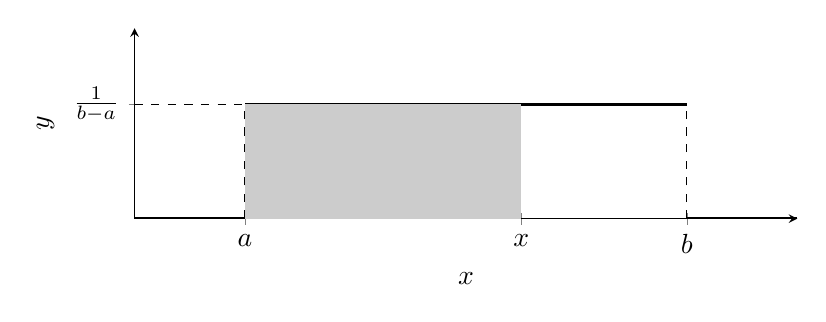
\begin{tikzpicture}

        \definecolor{siva}{rgb}{0.8, 0.8, 0.8}

        \begin{axis}[
            axis lines = left,
            xlabel = $x$,
            ylabel = {$y$},
            domain=-3:3,
            samples=100,
            height=4cm,
            width=10cm,
            xmin=-3, xmax=3,
            ymin=0, ymax=0.5,
            ytick={0.3},
            xtick={-2, 0.5, 2},
            yticklabels={$\frac{1}{b-a}$},
            xticklabels={$a$, $x$, $b$},
            yticklabel style={xshift=0cm}
        ]
        
        \draw[line width=1pt] (-3, 0) -- (-2, 0);
        \draw[line width=1pt] (-2, 0.3) -- (2, 0.3);
        \draw[line width=1pt] (2, 0) -- (3, 0);
    
        \draw[dashed] (-2, 0) -- (-2, 0.3);
        \draw[dashed] (2, 0) -- (2, 0.3);
        \draw[dashed] (-3, 0.3) -- (2, 0.3);
    
        \fill[siva] (-2,0) rectangle (0.5,0.3);
    
        \end{axis}
    \end{tikzpicture}
    $$
    F(x)=\int_{-\infty}^x p(t) \, d t= 
    \begin{cases}
        0, & \text{ če } x \leq a \\
        \frac{x-a}{b-a}, & \text{ če } a \leq x \leq b \\
        1, & \text{ če } x \geq b
    \end{cases}
    $$
    \item \emph{Normalna} ali \emph{Gaussova porazdelitev} $\operatorname{N}(\mu, \sigma)$, $(\mu \in \mathbb{R}, \sigma>0)$:
    $$
    p(x)=\frac{1}{\sigma \sqrt{2 \pi}} e^{-\frac{1}{2}\left(\frac{x-\mu}{\sigma}\right)^2}
    $$

    \begin{tikzpicture}
        \begin{axis}[
            axis lines = left,
            xlabel = $x$,
            ylabel = {$y$},
            domain=-3:3,
            samples=100,
            height=4cm,
            width=10cm,
            xmin=-3, xmax=3,
            ymin=0, ymax=0.5,
            xtick={0},
            xticklabels={$\mu$},
            yticklabels={}
        ]
        
        \addplot [black, thick] {1/(sqrt(2*pi))*exp(-(x^2/2)};
        \draw[dashed] (0, 0) -- (0, 0.3989);

        \end{axis}
    \end{tikzpicture}

    Če je $\sigma$ majhen: \hspace{5cm} Če je $\sigma$ velik:
    \begin{figure}[h]
        \begin{minipage}{0.45\textwidth}
            \centering
            \begin{tikzpicture}
                \begin{axis}[
                    axis lines = left,
                    xlabel = $x$,
                    ylabel = {$y$},
                    domain=-3:3,
                    samples=100,
                    height=4cm,
                    width=7cm,
                    xmin=-3, xmax=3,
                    ymin=0, ymax=1,
                    xtick={0},
                    xticklabels={$\mu$},
                    yticklabels={}
                ]
                
                \addplot [black, thick] {1/(sqrt(2*pi*0.22))*exp(-(x^2/(2*0.05))};
                \draw[dashed] (0, 0) -- (0, 0.8505);
        
                \end{axis}
            \end{tikzpicture}
        \end{minipage}
        \hfill
        \begin{minipage}{0.45\textwidth}
            \centering
            \begin{tikzpicture}
                \begin{axis}[
                    axis lines = left,
                    xlabel = $x$,
                    ylabel = {$y$},
                    domain=-3:3,
                    samples=100,
                    height=4cm,
                    width=7cm,
                    xmin=-3, xmax=3,
                    ymin=0, ymax=0.5,
                    xtick={0},
                    xticklabels={$\mu$},
                    yticklabels={}
                ]
                
                \addplot [black, thick] {1/(sqrt(2*pi*4))*exp(-(x^2/4)};
                \draw[dashed] (0, 0) -- (0, 0.1995);
        
                \end{axis}
            \end{tikzpicture}
        \end{minipage}
    \end{figure}

    $$
    F(x)=\frac{1}{\sigma \sqrt{2 \pi}} \int_{-\infty}^x e^{-\frac{1}{2}\left(\frac{x-\mu}{\sigma}\right)^2} \, d t \stackrel{\star}{=} \frac{1}{\sqrt{2 \pi}} \int_{-\infty}^{\frac{x-\mu}{\sigma}} e^{-\frac{1}{2}s^2} \, ds = \frac{1}{2}+\phi\left(\frac{x-\mu}{\sigma}\right)
    $$

    Kjer smo v enakosti $\star$ uvedli novo spremenljivko $s=\frac{t-\mu}{\sigma}$.
    
    \hspace{20pt} Tukaj je: $$\phi(x)=\frac{1}{\sqrt{2 \pi}} \int_0^x e^{2 \pi t^2} \, d t$$ \s

    $N(0,1)$: standardna normalna porazdelitev:
    $$
    p(x)=\frac{1}{\sqrt{2 \pi}} e^{-\frac{x^2}{2}}
    $$
    
    Laplaceova formula: za velike $n$ je:
    $$
    \operatorname{Bin}(n,p) \approx \operatorname{N}(np, \sqrt{npq})
    $$
    \begin{zgled}
        Sistolični krvni tlak je an populciji približno normalno porazdeljen: \s
        
        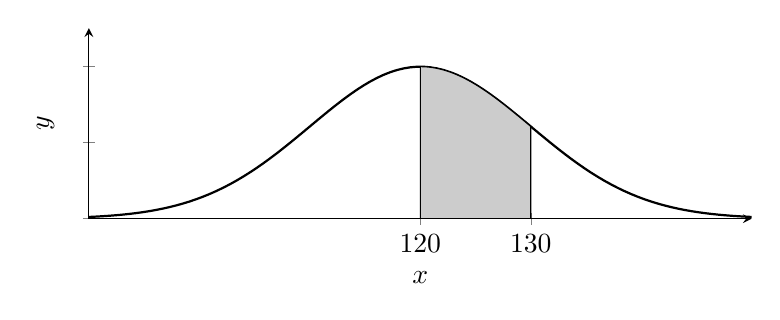
\begin{tikzpicture}

            \definecolor{siva}{rgb}{0.8, 0.8, 0.8}

            \begin{axis}[
                axis lines = left,
                xlabel = $x$,
                ylabel = {$y$},
                domain=-3:3,
                samples=100,
                height=4cm,
                width=10cm,
                xmin=-3, xmax=3,
                ymin=0, ymax=0.5,
                xtick={0, 1},
                xticklabels={120, 130},
                yticklabels={}
            ]
            
            \addplot [black, thick] {1/(sqrt(2*pi))*exp(-(x^2/2)};
            \addplot [fill=siva, domain=0:1] {1/(sqrt(2*pi))*exp(-(x^2/2)} \closedcycle;
            \draw[dashed] (0, 0) -- (0, 0.3989);
            \draw[dashed] (1, 0) -- (1, 0.2420);
        
            \end{axis}
        \end{tikzpicture}

        delež ljudi, ki imajo tlak med $120$ in $130 \operatorname{mm\ Hg}$.
    \end{zgled}

    \item \emph{Eksponenta porazdelitev} $\operatorname{Exp}(\lambda)$, $\lambda > 0$:
    $$
    p(x)= \begin{cases}\lambda e^{-\lambda x}, & \text { če } x \geq 0 \\ 0, & \text { sicer }\end{cases}
    $$

    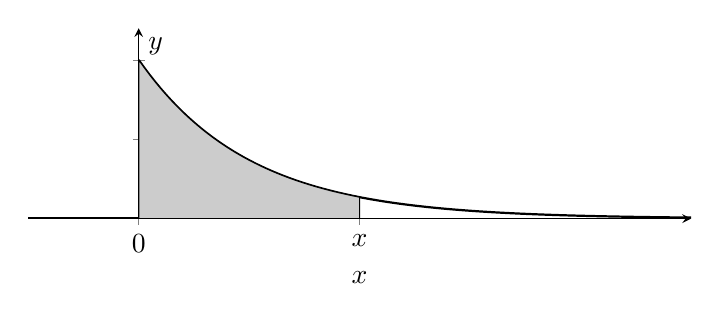
\begin{tikzpicture}

        \definecolor{siva}{rgb}{0.8, 0.8, 0.8}

        \begin{axis}[
            axis lines = left,
            xlabel = $x$,
            ylabel = {$y$},
            domain=0:5,
            samples=100,
            height=4cm,
            width=10cm,
            xmin=-1, xmax=5,
            ymin=0, ymax=1.2,
            axis y line=middle,
            xtick={0, 2},
            xticklabels={0, $x$},
            yticklabels={}
        ]
        
        \addplot [black, thick] {e^(-x)};
        \addplot [fill=siva, domain=0:2] {e^(-x)} \closedcycle;

        \draw[line width=1pt] (-1, 0) -- (0, 0);
        \draw[dashed] (0, 0) -- (0, 1);
        \draw[dashed] (2, 0) -- (2, 0.1353);
    
        \end{axis}
    \end{tikzpicture}

    $$
    F(x)= \begin{cases}1-e^{-\lambda x}, & \text { če } x \geq 0 \\ 0, & \text { sicer }\end{cases}
    $$

    \begin{tikzpicture}

        \definecolor{siva}{rgb}{0.8, 0.8, 0.8}

        \begin{axis}[
            axis lines = left,
            xlabel = $x$,
            ylabel = {$y$},
            domain=0:5,
            samples=100,
            height=4cm,
            width=10cm,
            xmin=-1, xmax=5,
            ymin=0, ymax=1.2,
            axis y line=middle,
            xtick={0, 2},
            ytick={1},
            xticklabels={0, $x$},
            yticklabels={1}
        ]
        
        \addplot [black, thick] {1-e^(-x)};

        \draw[line width=1pt] (-1, 0) -- (0, 0);
        \draw (2, 0) -- (2, 1-0.1353);
        \draw[dashed] (0, 1) -- (5, 1);
    
        \end{axis}
    \end{tikzpicture}

    \begin{zgled}
        Radioaktivni razpad - potreben čas, da se nekaj zgodi. 
    \end{zgled}

\end{enumerate}
\end{document}